\chapter{Séries temporais: estacionariedade e autocorrelação}
\label{cap:est}

\section{Por que séries temporais pedem ferramentas próprias}
Em corte transversal, observações independentes são razoáveis. Numa série, o valor de hoje depende do de ontem. Isso muda tudo: a mesma série é a nossa única amostra, e só podemos aprender com ela se o comportamento dela for, em algum sentido, estável ao longo do tempo. Essa estabilidade tem um nome: \textbf{estacionariedade}.

\section{Estacionariedade fraca}
Uma série $\{y_t\}$ é \textbf{fracamente estacionária} (ou estacionária em covariância) se
\begin{enumerate}[leftmargin=1.6em]
\item $\E(y_t)=\mu$ não depende de $t$;
\item $\Var(y_t)=\gamma_0$ não depende de $t$;
\item $\Cov(y_t,y_{t-k})=\gamma_k$ depende só da defasagem $k$, não de $t$.
\end{enumerate}
A \textbf{função de autocorrelação} (FAC) é $\rho_k=\gamma_k/\gamma_0$. A \textbf{FAC parcial} (FACP) em $k$ é a correlação entre $y_t$ e $y_{t-k}$ depois de descontar o efeito das defasagens intermediárias.

\begin{intuicao}[{FAC versus FACP}]
A FAC mistura efeitos diretos e indiretos: se hoje depende de ontem e ontem do anteontem, hoje e anteontem se correlacionam, mesmo sem ligação direta. A FACP tenta isolar só o elo direto.
\end{intuicao}

\section{Quatro séries que você precisa conhecer}
\begin{center}
\small
\begin{tabular}{p{3.2cm}p{4.1cm}p{6.4cm}}
\toprule
\textbf{Série} & \textbf{Definição} & \textbf{Propriedades} \\
\midrule
Ruído branco & $y_t=\varepsilon_t$, média 0, variância $\sigma^2$, sem correlação & $\rho_k=0$ para $k\ge1$. Bloco de construção de todos os modelos. \\
Passeio aleatório & $y_t=y_{t-1}+\varepsilon_t$ & \textbf{Não} estacionário: variância $t\sigma^2$ cresce. Choques são permanentes. \\
AR(1) & $y_t=\phi y_{t-1}+\varepsilon_t$ & Estacionário se $|\phi|<1$; $\rho_k=\phi^k$ (decaimento geométrico). \\
MA(1) & $y_t=\varepsilon_t+\theta\varepsilon_{t-1}$ & Sempre estacionário; $\rho_1=\theta/(1+\theta^2)$ e $\rho_k=0$ para $k\ge2$. \\
\bottomrule
\end{tabular}
\end{center}

\begin{atencao}[{Armadilha: o sinal do MA muda de livro para livro}]
Este guia usa $y_t=\varepsilon_t+\theta\varepsilon_{t-1}$ (sinal \textbf{positivo}), como Hamilton, o \texttt{arima} do R e o \texttt{statsmodels}. Cryer e Chan e Mills usam o sinal \textbf{negativo}, $y_t=\varepsilon_t-\theta\varepsilon_{t-1}$, herdado de Box e Jenkins. Com a convenção negativa, $\rho_1=-\theta/(1+\theta^2)$. Se você copiar uma fórmula de um livro e um coeficiente de um software sem checar a convenção, o sinal do $\theta$ sai trocado. Ao ler uma saída de software, confirme sempre qual convenção ele adota.
\end{atencao}

\begin{simulacao}[{Conferido: MA(1) com coeficiente 0{,}5}]
A fórmula dá $\rho_1=0{,}5/1{,}25=0{,}4$. A autocorrelação teórica calculada pelo \texttt{statsmodels} é $0{,}4$. Note também que $\theta=2$ dá $2/5=0{,}4$: \textbf{dois valores de $\theta$ (um e seu inverso) geram a mesma FAC}. Por isso exige-se invertibilidade, $|\theta|<1$, para identificar o modelo. E o máximo de $|\rho_1|$ num MA(1) é $0{,}5$.
\end{simulacao}

\section{AR(2) e a condição de estacionariedade}
Para $y_t=\phi_1y_{t-1}+\phi_2y_{t-2}+\varepsilon_t$, as três condições abaixo são equivalentes a ``raízes do polinômio fora do círculo unitário'' (o chamado triângulo de estacionariedade):
\[
\phi_1+\phi_2<1,\qquad \phi_2-\phi_1<1,\qquad |\phi_2|<1.
\]
As equações de Yule--Walker dão $\rho_1=\phi_1/(1-\phi_2)$ e $\rho_k=\phi_1\rho_{k-1}+\phi_2\rho_{k-2}$ para $k\ge2$.

\begin{simulacao}[{Conferido: AR(2) com coeficientes 0{,}5 e 0{,}3}]
Yule--Walker: $\rho_1=0{,}5/0{,}7=0{,}7143$ e $\rho_2=0{,}5\times0{,}7143+0{,}3=0{,}6571$. O \texttt{statsmodels} dá os mesmos valores. Testei também cinco pares $(\phi_1,\phi_2)$ por cálculo das raízes: $(0{,}5;0{,}3)$ é estacionário; $(1{,}2;-0{,}2)$, $(0{,}5;0{,}6)$, $(1{,}0;0)$ e $(-0{,}5;0{,}5)$ não são, o que coincide com o triângulo.
\end{simulacao}

\section{Assinaturas na FAC e na FACP}
\begin{center}
\small
\begin{tabular}{lcc}
\toprule
\textbf{Modelo} & \textbf{FAC} & \textbf{FACP} \\
\midrule
AR($p$) & decai gradualmente & \textbf{corta} depois de $p$ \\
MA($q$) & \textbf{corta} depois de $q$ & decai gradualmente \\
ARMA($p,q$) & decai & decai \\
\bottomrule
\end{tabular}
\end{center}

\begin{center}
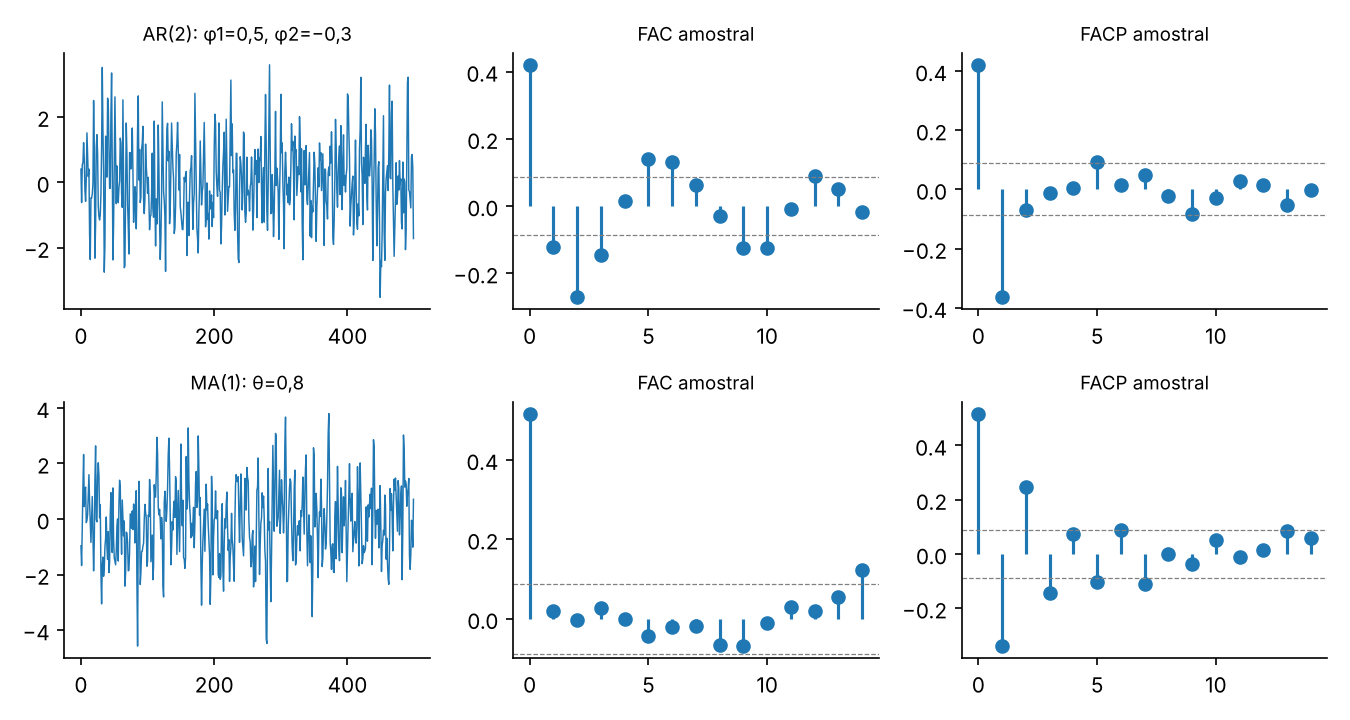
\includegraphics[width=\textwidth]{fig/acf_pacf.png}\\
\small Séries simuladas (500 pontos) e suas FAC e FACP amostrais. Linha de cima: AR(2) ($\phi_1=0{,}5$, $\phi_2=-0{,}3$): a FACP corta em 2. Linha de baixo: MA(1) ($\theta=0{,}8$): a FAC corta em 1. As linhas pontilhadas são as bandas $\pm1{,}96/\sqrt n$.
\end{center}

\begin{atencao}
As bandas $\pm1{,}96/\sqrt n$ valem sob a hipótese de ruído branco. Para uma série que \emph{não} é ruído branco, as bandas corretas (de Bartlett) são mais largas, e em amostras curtas a FAC amostral é viesada para baixo. Interprete os gráficos como pista, não como veredito.
\end{atencao}

\begin{exercicio}
Num AR(1) com $\phi=0{,}6$ e $\sigma^2=1$, calcule $\gamma_0$, $\rho_1$ e $\rho_3$.
\end{exercicio}
\sol{$\gamma_0=\sigma^2/(1-\phi^2)=1/0{,}64=1{,}5625$. $\rho_1=0{,}6$ e $\rho_3=0{,}6^3=0{,}216$.}

\begin{exercicio}
Um MA(1) tem $\theta=-0{,}4$ (convenção positiva). Qual é $\rho_1$? E se a convenção do livro fosse a negativa, com o mesmo número $-0{,}4$ impresso?
\end{exercicio}
\sol{Convenção positiva: $\rho_1=-0{,}4/(1+0{,}16)=-0{,}345$. Convenção negativa, com $\theta=-0{,}4$: $\rho_1=-\theta/(1+\theta^2)=+0{,}345$. O mesmo número com convenções diferentes dá correlações de sinais opostos.}
